\appendix

\chapter{Appendix of Figures} 

\pagebreak


\section{\boldmath Two components, $\tau_1 = 150$ps, $\tau_2=190$-$250$ps\unboldmath\label{t1-150}}

\begin{minipage}{ .47\linewidth}
    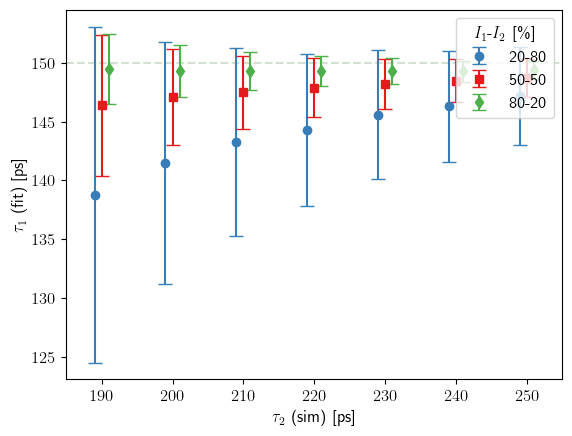
\includegraphics[width=\linewidth]{Batch 3/regular IRF/tau1 150/output/plotfin/t1.png}
    \captionof{figure}{Fitted $\tau_1$}
    \label{fig:150-t1}
\end{minipage}
\hfill
\begin{minipage}{ .47\linewidth}
    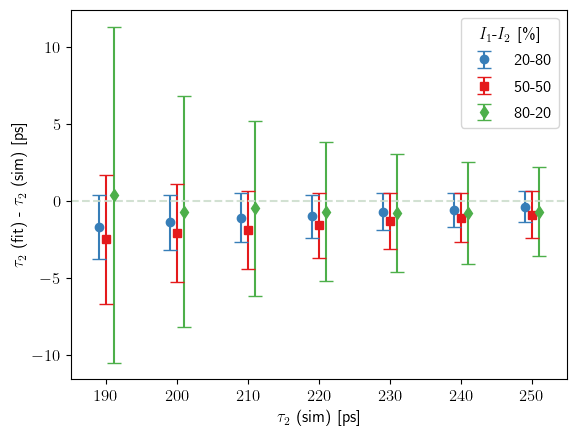
\includegraphics[width=\linewidth]{Batch 3/regular IRF/tau1 150/output/plotfin/t2.png}
    \captionof{figure}{$\tau_2$ (Fitted$-$Simulated)}
    \label{fig:150-t2}
\end{minipage}
\begin{minipage}{ .47\linewidth}
    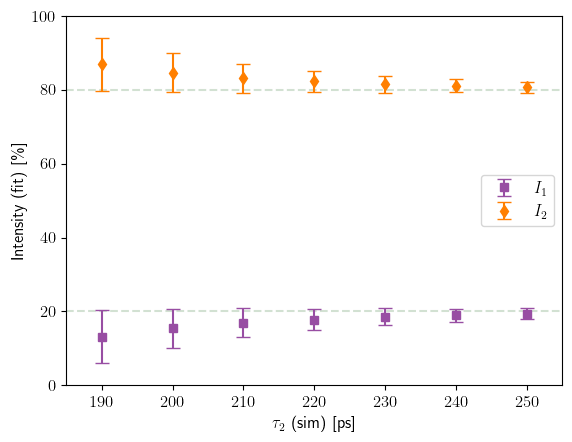
\includegraphics[width=\linewidth]{Batch 3/regular IRF/tau1 150/output/plotfin/2080.png}
    \captionof{figure}{$I_1 = 20\%, I_2 = 80\%$}
    \label{fig:150-2080}
\end{minipage}
\hfill
\begin{minipage}{ .47\linewidth}
    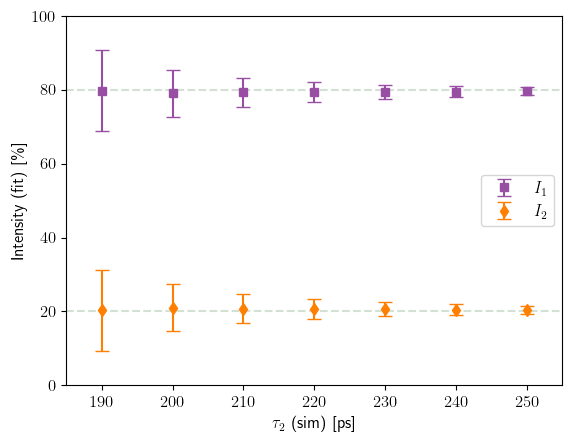
\includegraphics[width=\linewidth]{Batch 3/regular IRF/tau1 150/output/plotfin/8020.png}
    \captionof{figure}{$I_1 = 80\%, I_2 = 20\%$}
    \label{fig:150-8020}
\end{minipage}
\begin{minipage}{\linewidth}
    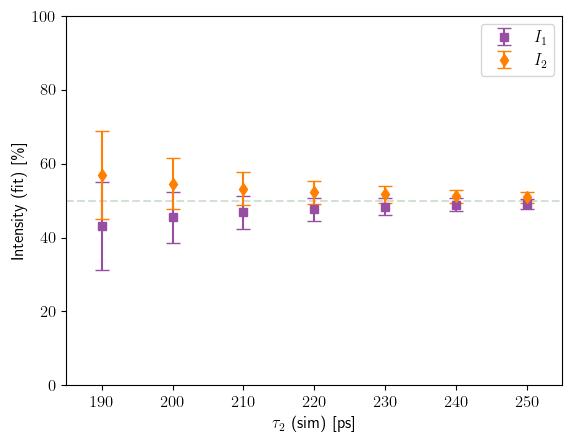
\includegraphics[width= .47\linewidth]{Batch 3/regular IRF/tau1 150/output/plotfin/5050.png}
    \captionof{figure}{$I_1 = 50\%, I_2 = 50\%$}
    \label{fig:150-5050}
\end{minipage}

\section{\boldmath Two components, $\tau_1 = 220$ps, $\tau_2=260$-$340$ps\unboldmath\label{t1-220}}

\begin{minipage}{ .47\linewidth}
    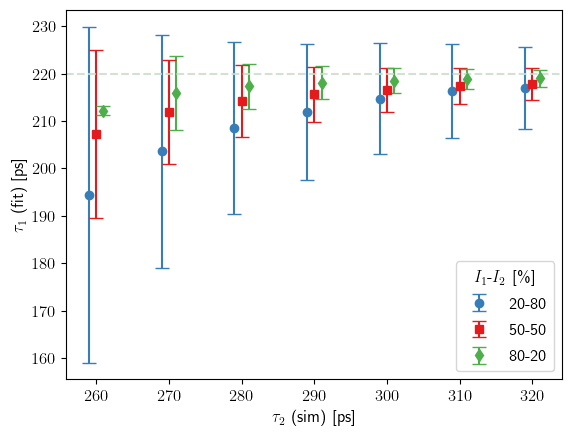
\includegraphics[width=\linewidth]{Batch 3/regular IRF/tau1 220/output/plotfin/t1.png}
    \captionof{figure}{Fitted $\tau_1$}
    \label{fig:220-t1}
\end{minipage}
\hfill
\begin{minipage}{ .47\linewidth}
    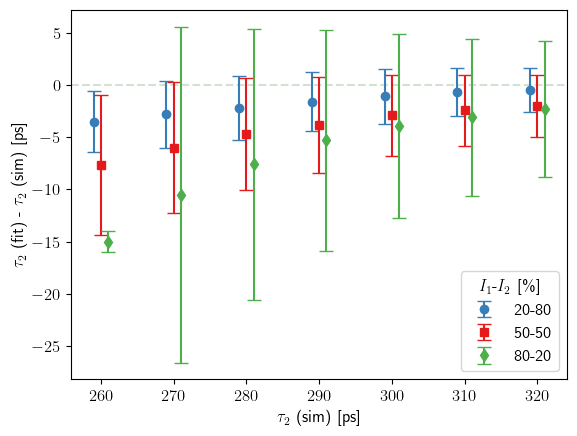
\includegraphics[width=\linewidth]{Batch 3/regular IRF/tau1 220/output/plotfin/t2.png}
    \captionof{figure}{$\tau_2$ (Fitted$-$Simulated)}
    \label{fig:220-t2}
\end{minipage}
\begin{minipage}{ .47\linewidth}
    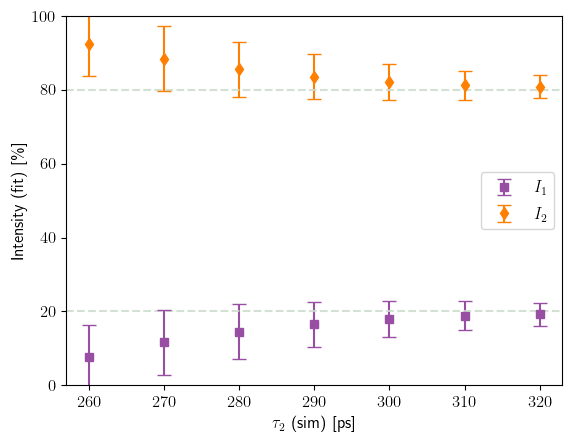
\includegraphics[width=\linewidth]{Batch 3/regular IRF/tau1 220/output/plotfin/2080.png}
    \captionof{figure}{$I_1 = 20\%, I_2 = 80\%$}
    \label{fig:220-2080}
\end{minipage}
\hfill
\begin{minipage}{ .47\linewidth}
     
    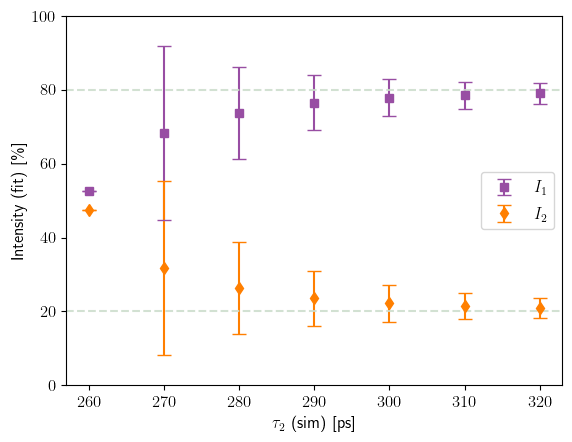
\includegraphics[width=\linewidth]{Batch 3/regular IRF/tau1 220/output/plotfin/8020.png}
    \captionof{figure}{$I_1 = 80\%, I_2 = 20\%$}
    \label{fig:220-8020}
\end{minipage}
\begin{minipage}{\linewidth}
     
    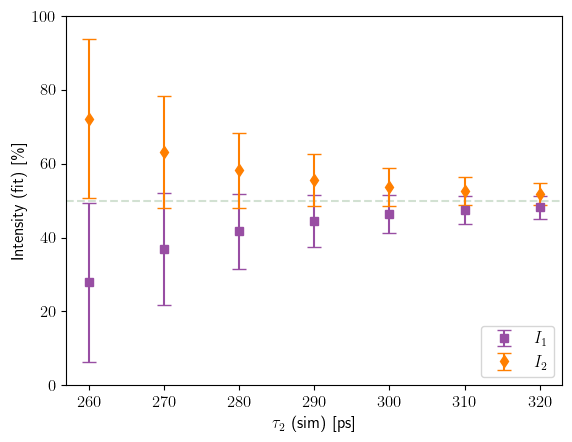
\includegraphics[width= .47\linewidth]{Batch 3/regular IRF/tau1 220/output/plotfin/5050.png}
    \captionof{figure}{$I_1 = 50\%, I_2 = 50\%$}
    \label{fig:220-5050}
\end{minipage}

\section{\boldmath Comparison two component fit, $\tau_1 = 150,180,220$ \unboldmath \label{comp-t1}}


{\centering \textbf{First component, $\tau_1$}

\begin{minipage}{.47\linewidth}
     
    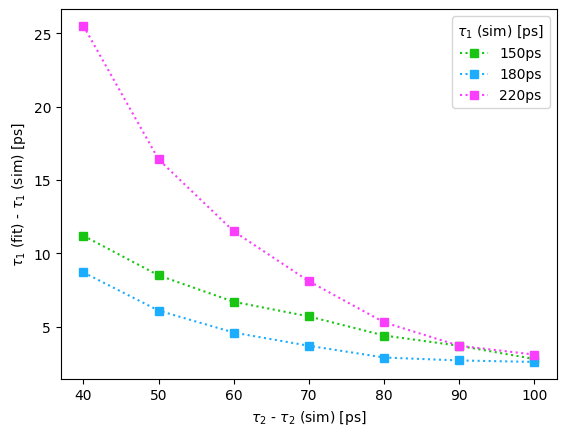
\includegraphics[width=\linewidth]{Batch 3/regular IRF/t1-diff 2080.png}
    \captionof{figure}{$I_1$-$I_2=20\%$-$80\%$}
    \label{fig:comp-t1-2080}
\end{minipage}
\hfill
\begin{minipage}{.47\linewidth}
     
    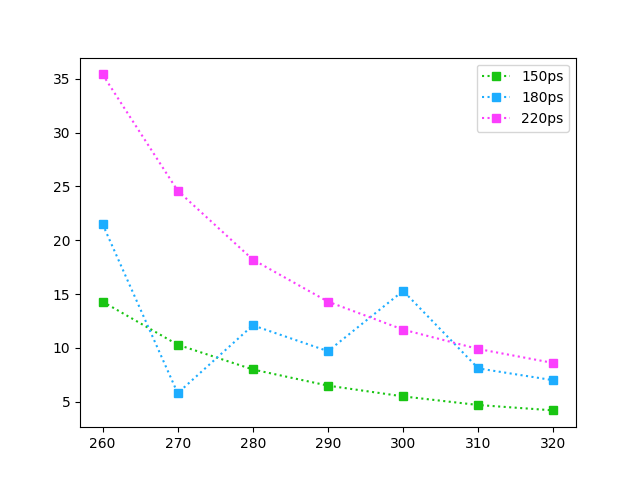
\includegraphics[width=\linewidth]{Batch 3/regular IRF/t1-err 2080.png}
    \captionof{figure}{Std. dev. $I_1$-$I_2=20\%$-$80\%$}
    \label{fig:comp-t1err-2080}
\end{minipage}
\begin{minipage}{.47\linewidth}
     
    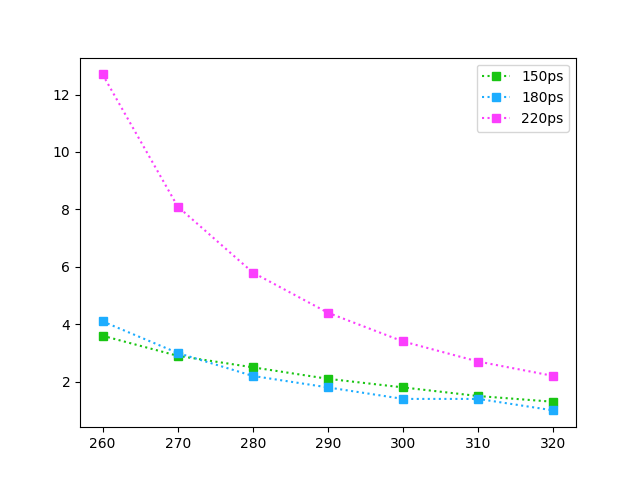
\includegraphics[width=\linewidth]{Batch 3/regular IRF/t1-diff 5050.png}
    \captionof{figure}{$I_1$-$I_2=50\%$-$50\%$}
    \label{fig:comp-t1-5050}
\end{minipage}
\hfill
\begin{minipage}{.47\linewidth}
    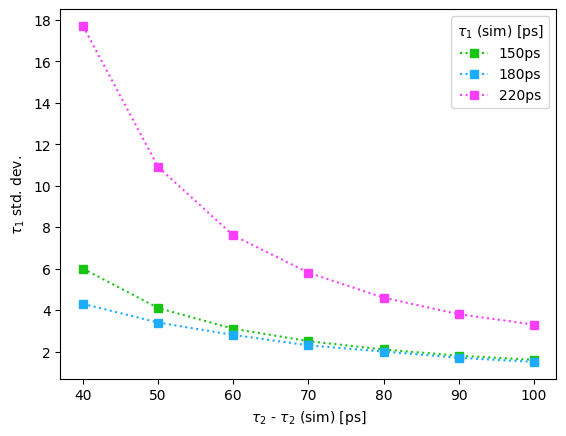
\includegraphics[width=\linewidth]{Batch 3/regular IRF/t1-err 5050.png}
    \captionof{figure}{Std. dev. $I_1$-$I_2=50\%$-$50\%$}
    \label{fig:comp-t1err-5050}
\end{minipage}
\begin{minipage}{.47\linewidth}
    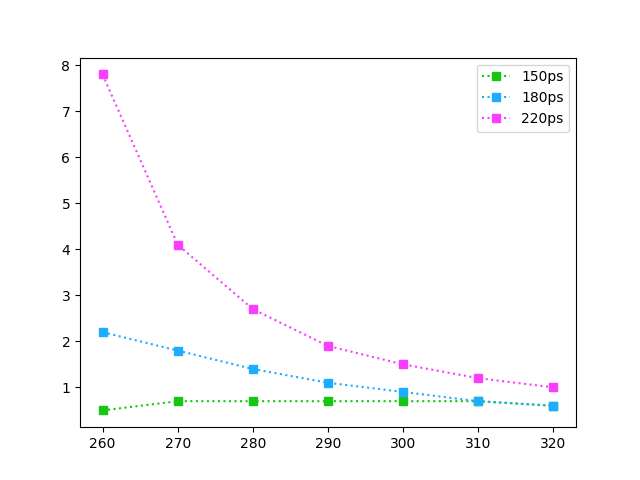
\includegraphics[width=\linewidth]{Batch 3/regular IRF/t1-diff 8020.png}
    \captionof{figure}{$I_1$-$I_2=80\%$-$20\%$}
    \label{fig:comp-t1-8020}
\end{minipage}
\hfill
\begin{minipage}{.47\linewidth}
    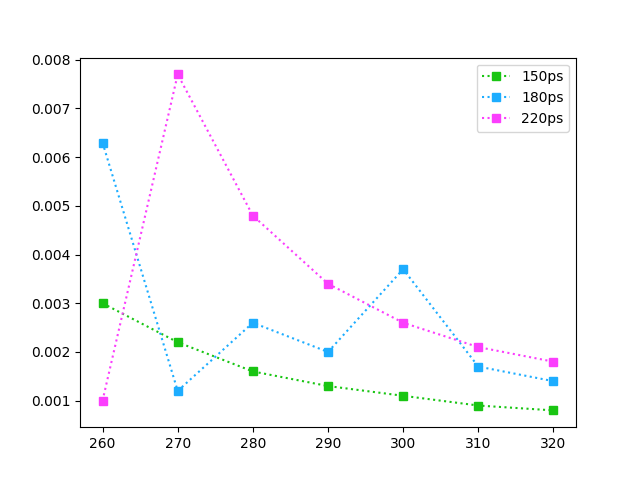
\includegraphics[width=\linewidth]{Batch 3/regular IRF/t1-err 8020.png}
    \captionof{figure}{Std. dev. $I_1$-$I_2=80\%$-$20\%$}
    \label{fig:comp-t1err-8020}
\end{minipage}


\textbf{Second component, $\tau_2$}

\begin{minipage}{.47\linewidth}
    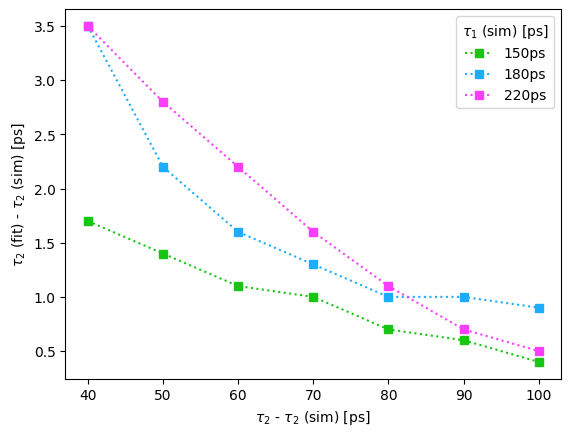
\includegraphics[width=\linewidth]{Batch 3/regular IRF/t2-diff 2080.png}
    \captionof{figure}{$I_1$-$I_2=20\%$-$80\%$}
    \label{fig:comp-t2-2080}
\end{minipage}
\hfill
\begin{minipage}{.47\linewidth}
    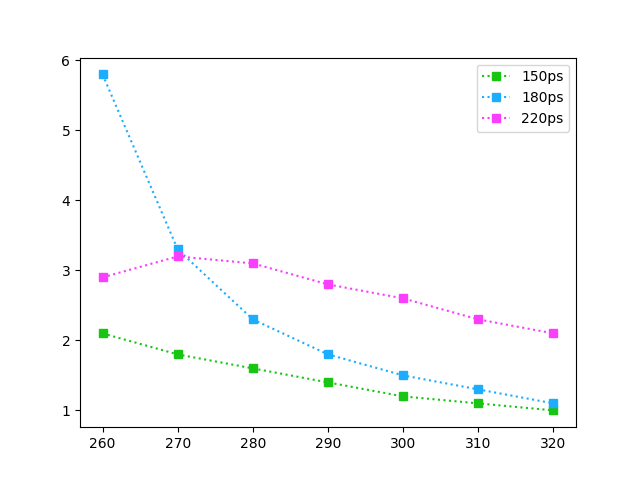
\includegraphics[width=\linewidth]{Batch 3/regular IRF/t2-err 2080.png}
    \captionof{figure}{Std. dev. $I_1$-$I_2=20\%$-$80\%$}
    \label{fig:comp-t2err-2080}
\end{minipage}
\begin{minipage}{.47\linewidth}
    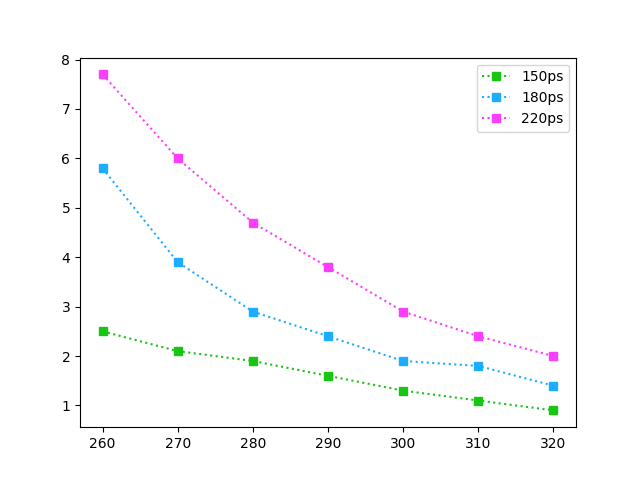
\includegraphics[width=\linewidth]{Batch 3/regular IRF/t2-diff 5050.png}
    \captionof{figure}{$I_1$-$I_2=50\%$-$50\%$}
    \label{fig:comp-t2-5050}
\end{minipage}
\hfill
\begin{minipage}{.47\linewidth}
    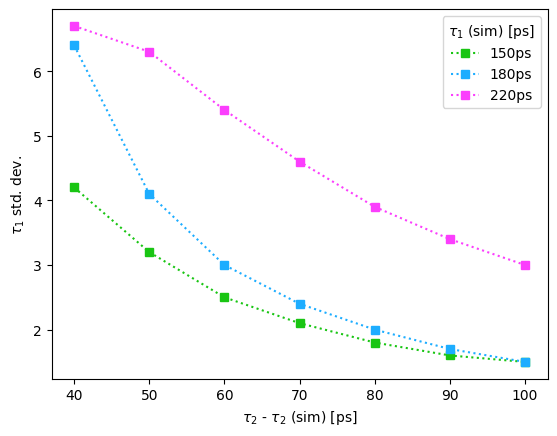
\includegraphics[width=\linewidth]{Batch 3/regular IRF/t2-err 5050.png}
    \captionof{figure}{Std. dev. $I_1$-$I_2=50\%$-$50\%$}
    \label{fig:comp-t2err-5050}
\end{minipage}
\begin{minipage}{.47\linewidth}
    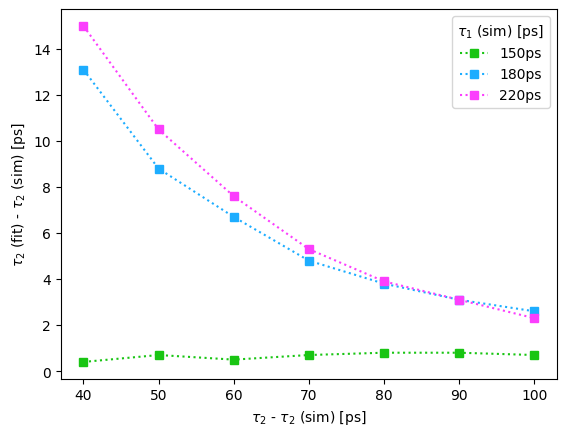
\includegraphics[width=\linewidth]{Batch 3/regular IRF/t2-diff 8020.png}
    \captionof{figure}{$I_1$-$I_2=80\%$-$20\%$}
    \label{fig:comp-t2-8020}
\end{minipage}
\hfill
\begin{minipage}{.47\linewidth}
    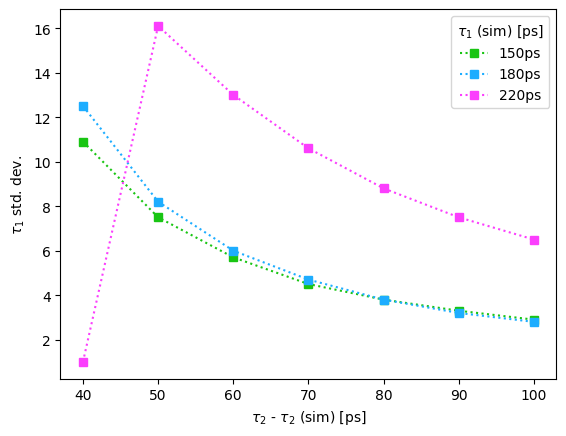
\includegraphics[width=\linewidth]{Batch 3/regular IRF/t2-err 8020.png}
    \captionof{figure}{Std. dev. $I_1$-$I_2=80\%$-$20\%$}
    \label{fig:comp-t2err-8020}
\end{minipage}

\pagebreak
\textbf{Intensity}

\begin{minipage}{.47\linewidth}
    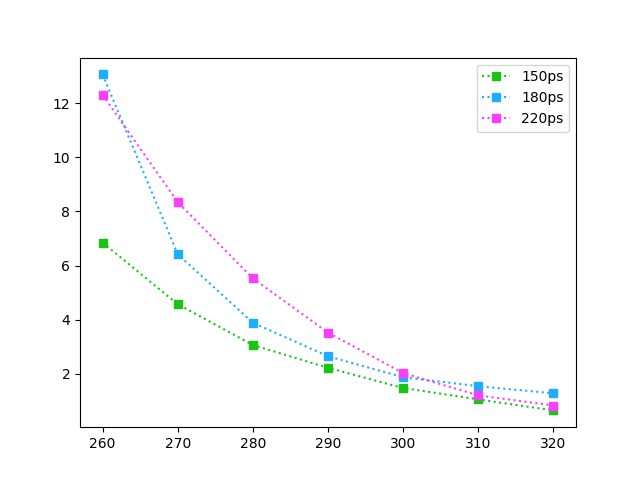
\includegraphics[width=\linewidth]{Batch 3/regular IRF/2080-diff i1.png}
    \captionof{figure}{$I_1$-$I_2=20\%$-$80\%$}
    \label{fig:comp-I-2080}
\end{minipage}
\hfill
\begin{minipage}{.47\linewidth}
    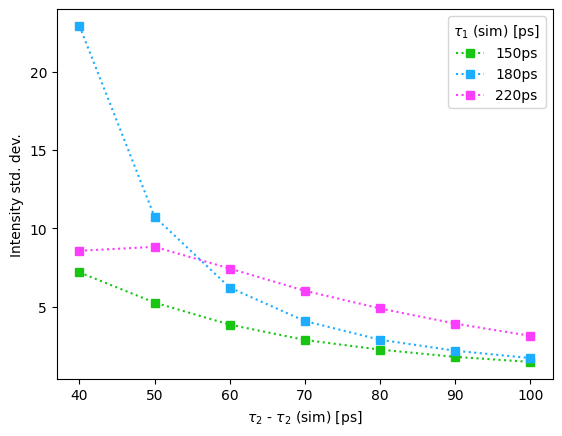
\includegraphics[width=\linewidth]{Batch 3/regular IRF/2080-err i1.png}
    \captionof{figure}{Std. dev. $I_1$-$I_2=20\%$-$80\%$}
    \label{fig:comp-Ierr-2080}
\end{minipage}
\begin{minipage}{.47\linewidth}
    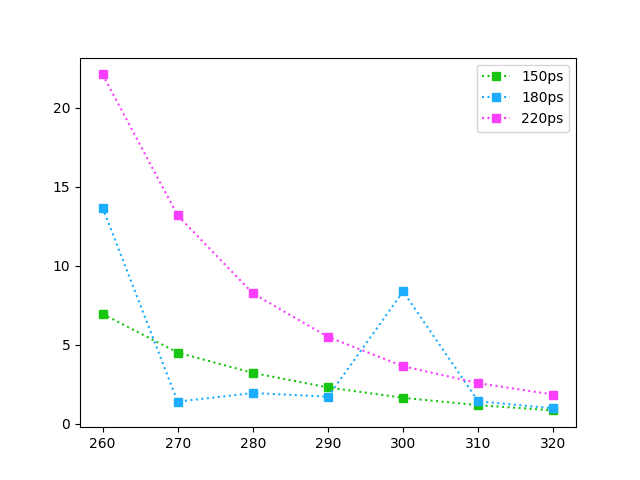
\includegraphics[width=\linewidth]{Batch 3/regular IRF/5050-diff i1.png}
    \captionof{figure}{$I_1$-$I_2=50\%$-$50\%$}
    \label{fig:comp-I-5050}
\end{minipage}
\hfill
\begin{minipage}{.47\linewidth}
    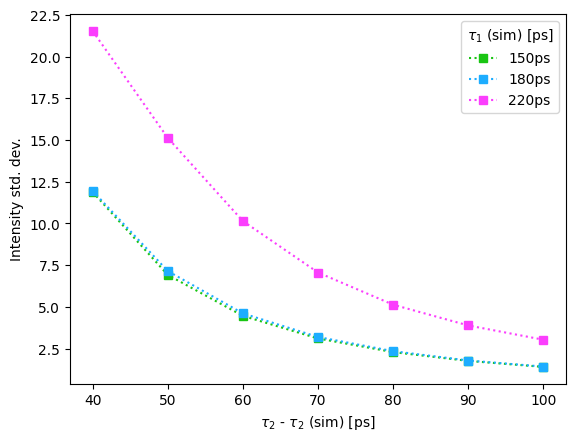
\includegraphics[width=\linewidth]{Batch 3/regular IRF/5050-err i1.png}
    \captionof{figure}{Std. dev. $I_1$-$I_2=50\%$-$50\%$}
    \label{fig:comp-Ierr-5050}
\end{minipage}
\begin{minipage}{.47\linewidth}
    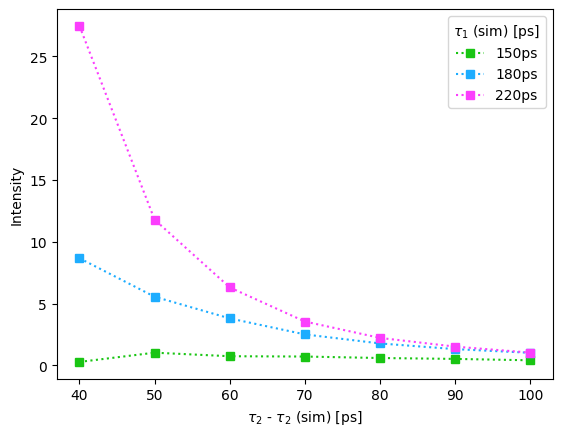
\includegraphics[width=\linewidth]{Batch 3/regular IRF/8020-diff i1.png}
    \captionof{figure}{$I_1$-$I_2=80\%$-$20\%$}
    \label{fig:comp-I-8020}
\end{minipage}
\hfill
\begin{minipage}{.47\linewidth}
    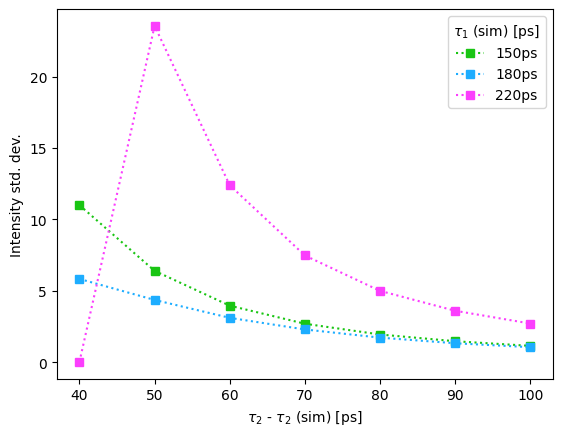
\includegraphics[width=\linewidth]{Batch 3/regular IRF/8020-err i1.png}
    \captionof{figure}{Std. dev. $I_1$-$I_2=80\%$-$20\%$}
    \label{fig:comp-Ierr-8020}
\end{minipage}

\section{\boldmath Two components, Single Gaussian IRF, $\tau_1 = 150$ps, $\tau_2=180$-$230$ps\unboldmath\label{1g}}

\begin{minipage}{ .47\linewidth}
    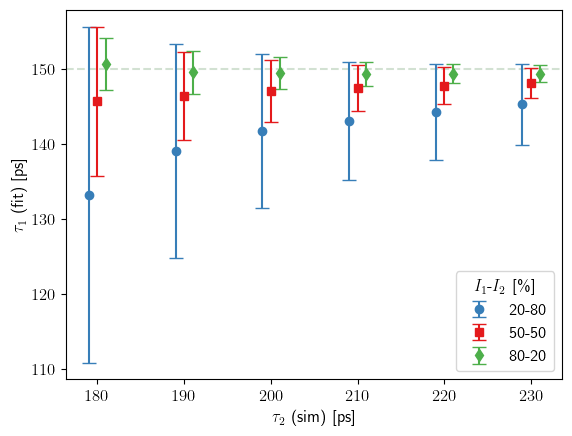
\includegraphics[width=\linewidth]{Batch 3/single Gaussian IRF/gauss210/150/output/plotfin/t1.png}
    \captionof{figure}{Fitted $\tau_1$}
    \label{fig:1g-t1}
\end{minipage}
\hfill
\begin{minipage}{ .47\linewidth}
    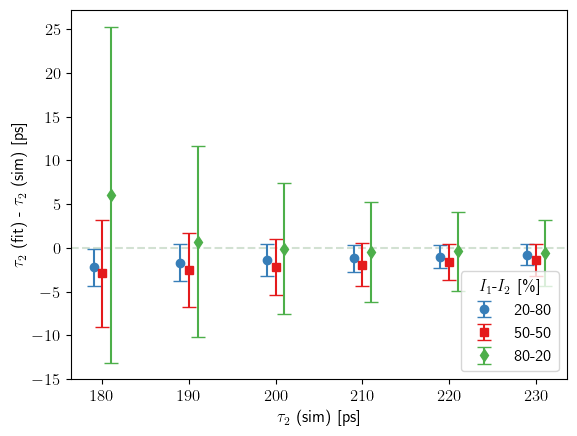
\includegraphics[width=\linewidth]{Batch 3/single Gaussian IRF/gauss210/150/output/plotfin/t2.png}
    \captionof{figure}{$\tau_2$ (Fitted$-$Simulated)}
    \label{fig:1g-t2}
\end{minipage}
\begin{minipage}{ .47\linewidth}
    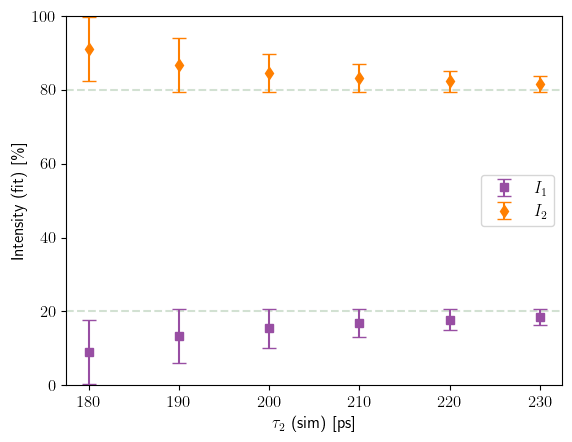
\includegraphics[width=\linewidth]{Batch 3/single Gaussian IRF/gauss210/150/output/plotfin/2080.png}
    \captionof{figure}{$I_1 = 20\%, I_2 = 80\%$}
    \label{fig:1g-2080}
\end{minipage}
\hfill
\begin{minipage}{ .47\linewidth}
    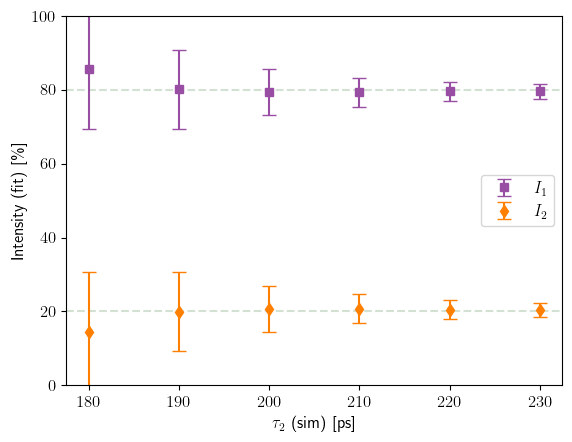
\includegraphics[width=\linewidth]{Batch 3/single Gaussian IRF/gauss210/150/output/plotfin/8020.png}
    \captionof{figure}{$I_1 = 80\%, I_2 = 20\%$}
    \label{fig:1g-8020}
\end{minipage}
\begin{minipage}{\linewidth}
    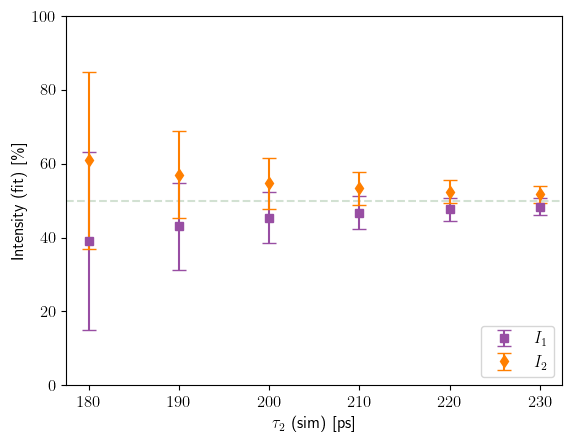
\includegraphics[width= .47\linewidth]{Batch 3/single Gaussian IRF/gauss210/150/output/plotfin/5050.png}
    \captionof{figure}{$I_1 = 50\%, I_2 = 50\%$}
    \label{fig:1g-5050}
\end{minipage}


\section{\boldmath Comparison two component fit, single IRF, FWHM = 210,180,150,100\unboldmath\label{comp-irf}}

\textbf{First component, $\tau_1$}

\begin{minipage}{.47\linewidth}
     
    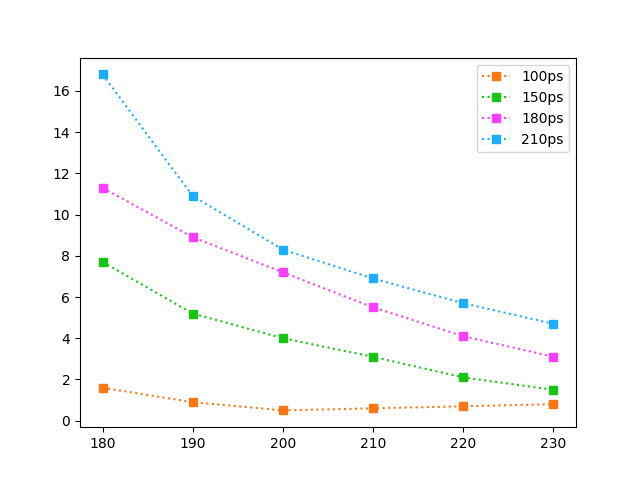
\includegraphics[width=\linewidth]{Batch 3/single Gaussian IRF/t1-diff 2080.png}
    \captionof{figure}{$I_1$-$I_2=20\%$-$80\%$}
    \label{fig:compirf-t1-2080}
\end{minipage}
\hfill
\begin{minipage}{.47\linewidth}
     
    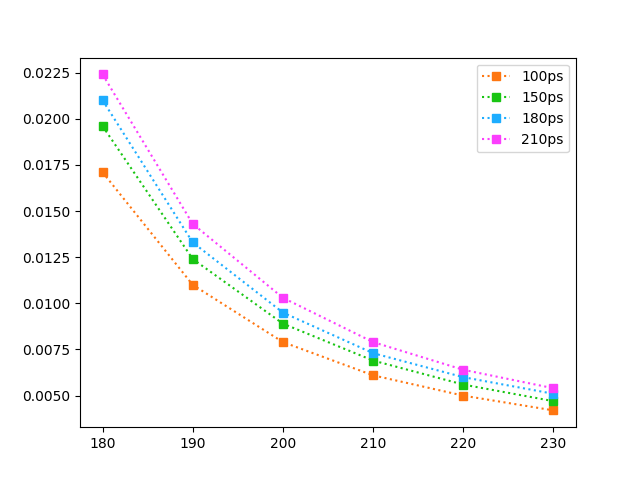
\includegraphics[width=\linewidth]{Batch 3/single Gaussian IRF/t1-err 2080.png}
    \captionof{figure}{Std. dev. $I_1$-$I_2=20\%$-$80\%$}
    \label{fig:compirf-t1err-2080}
\end{minipage}
\begin{minipage}{.47\linewidth}
     
    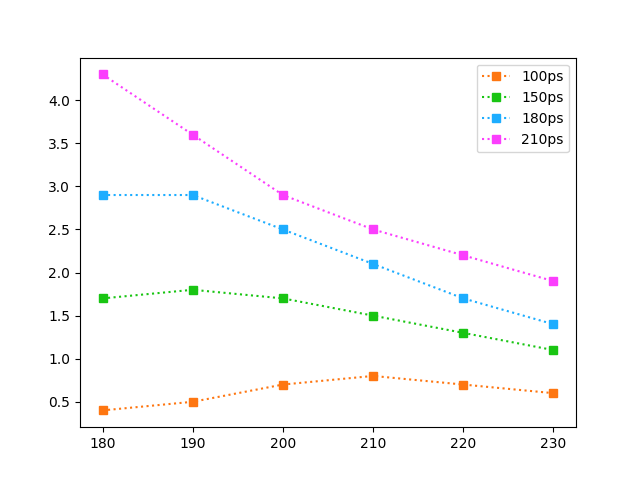
\includegraphics[width=\linewidth]{Batch 3/single Gaussian IRF/t1-diff 5050.png}
    \captionof{figure}{$I_1$-$I_2=50\%$-$50\%$}
    \label{fig:compirf-t1-5050}
\end{minipage}
\hfill
\begin{minipage}{.47\linewidth}
     
    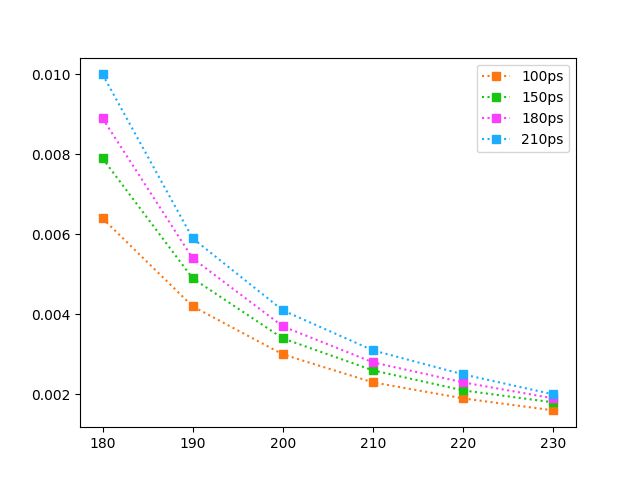
\includegraphics[width=\linewidth]{Batch 3/single Gaussian IRF/t1-err 5050.png}
    \captionof{figure}{Std. dev. $I_1$-$I_2=50\%$-$50\%$}
    \label{fig:compirf-t1err-5050}
\end{minipage}
\begin{minipage}{.47\linewidth}
     
    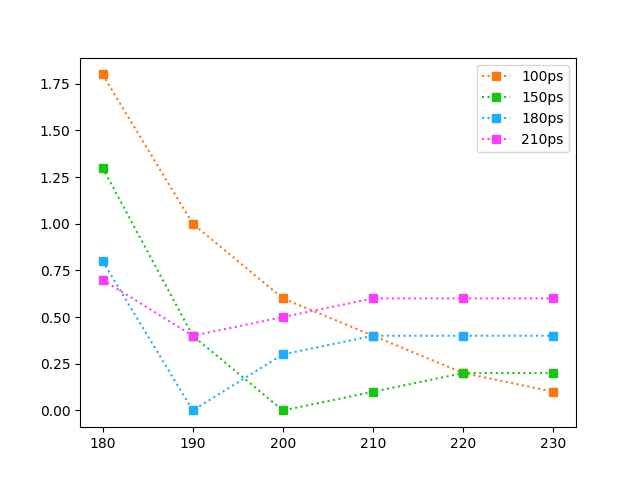
\includegraphics[width=\linewidth]{Batch 3/single Gaussian IRF/t1-diff 8020.png}
    \captionof{figure}{$I_1$-$I_2=80\%$-$20\%$}
    \label{fig:compirf-t1-8020}
\end{minipage}
\hfill
\begin{minipage}{.47\linewidth}
     
    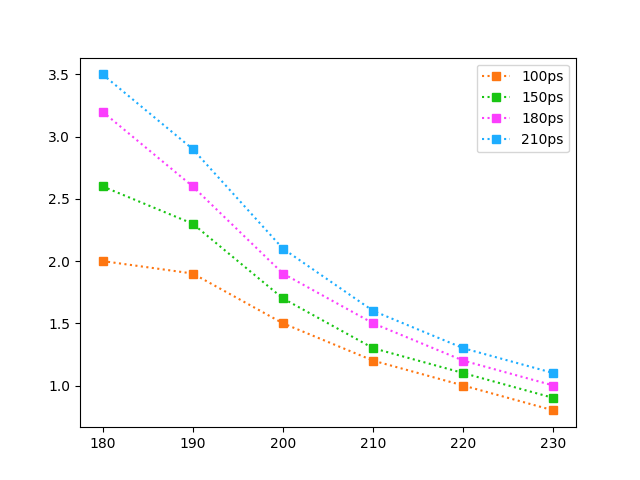
\includegraphics[width=\linewidth]{Batch 3/single Gaussian IRF/t1-err 8020.png}
    \captionof{figure}{Std. dev. $I_1$-$I_2=80\%$-$20\%$}
    \label{fig:compirf-t1err-8020}
\end{minipage}

\vfill
\textbf{Second component$\tau_2$}

\begin{minipage}{ .47\linewidth}
    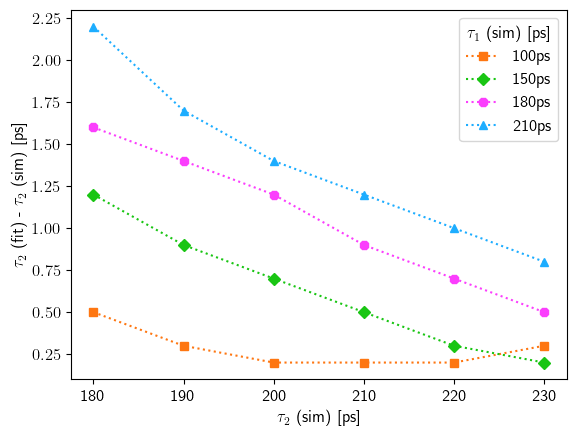
\includegraphics[width=\linewidth]{Batch 3/single Gaussian IRF/t2-diff 2080.png}
    \captionof{figure}{$I_1$-$I_2=20\%$-$80\%$}
    \label{fig:compirf-t2-2080}
\end{minipage}
\hfill
\begin{minipage}{ .47\linewidth}
    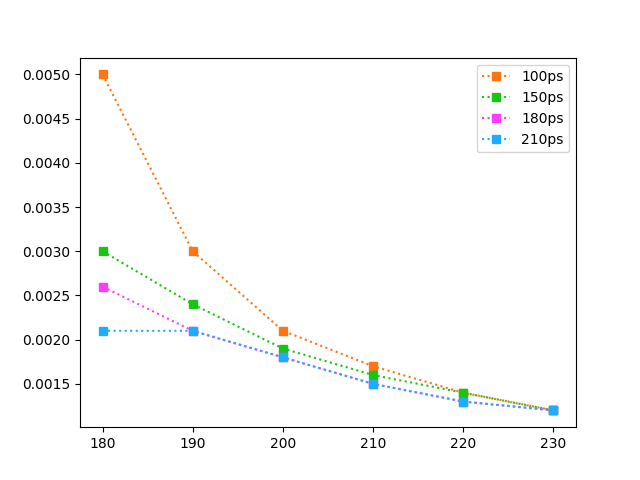
\includegraphics[width=\linewidth]{Batch 3/single Gaussian IRF/t2-err 2080.png}
    \captionof{figure}{Std. dev. $I_1$-$I_2=20\%$-$80\%$}
    \label{fig:compirf-t2err-2080}
\end{minipage}
\begin{minipage}{ .47\linewidth}
    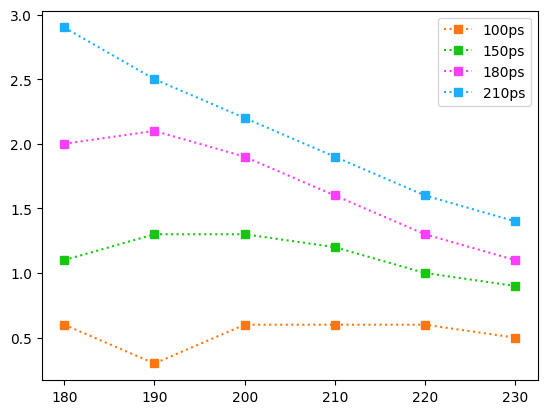
\includegraphics[width=\linewidth]{Batch 3/single Gaussian IRF/t2-diff 5050.png}
    \captionof{figure}{$I_1$-$I_2=50\%$-$50\%$}
    \label{fig:compirf-t2-5050}
\end{minipage}
\hfill
\begin{minipage}{ .47\linewidth}
    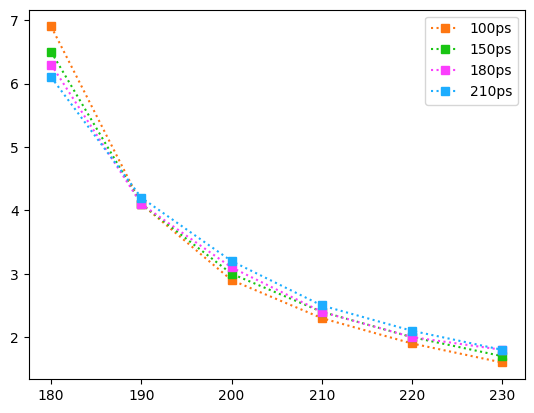
\includegraphics[width=\linewidth]{Batch 3/single Gaussian IRF/t2-err 5050.png}
    \captionof{figure}{Std. dev. $I_1$-$I_2=50\%$-$50\%$}
    \label{fig:compirf-t2err-5050}
\end{minipage}
\begin{minipage}{ .47\linewidth}
    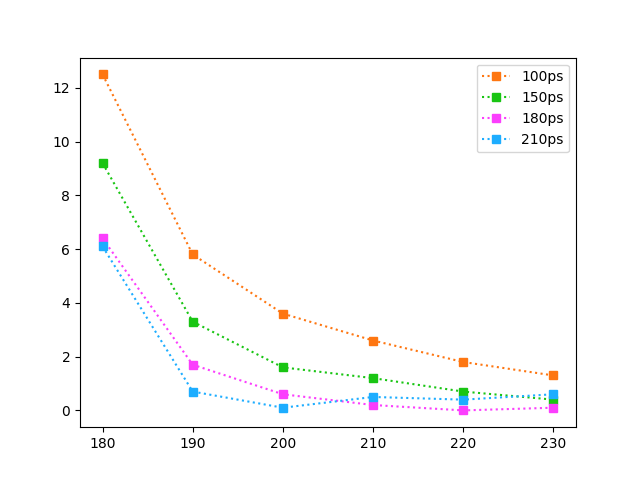
\includegraphics[width=\linewidth]{Batch 3/single Gaussian IRF/t2-diff 8020.png}
    \captionof{figure}{$I_1$-$I_2=80\%$-$20\%$}
    \label{fig:compirf-t2-8020}
\end{minipage}
\hfill
\begin{minipage}{ .47\linewidth}
    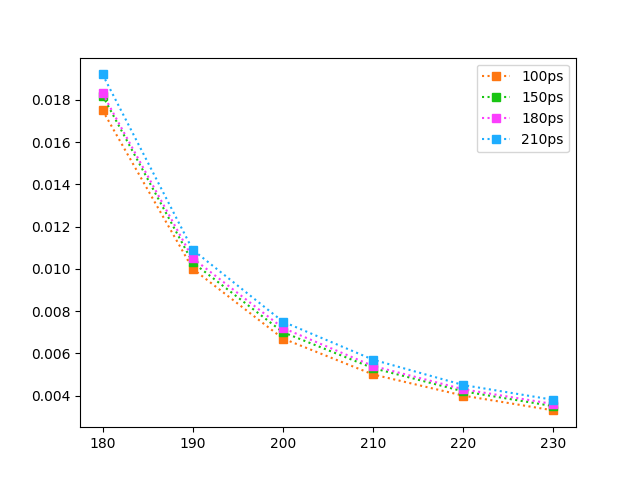
\includegraphics[width=\linewidth]{Batch 3/single Gaussian IRF/t2-err 8020.png}
    \captionof{figure}{Std. dev. $I_1$-$I_2=80\%$-$20\%$}
    \label{fig:compirf-t2err-8020}
\end{minipage}

\pagebreak
\textbf{Intensity}

\begin{minipage}{ .47\linewidth}
    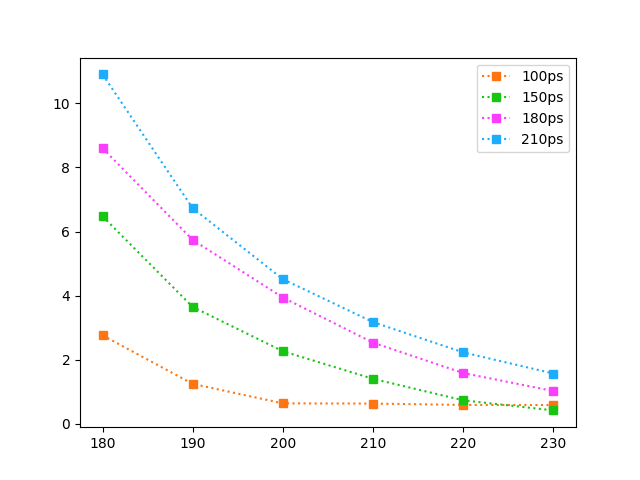
\includegraphics[width=\linewidth]{Batch 3/single Gaussian IRF/2080-diff i1.png}
    \captionof{figure}{$I_1$-$I_2=20\%$-$80\%$}
    \label{fig:compirf-I-2080}
\end{minipage}
\hfill
\begin{minipage}{ .47\linewidth}
    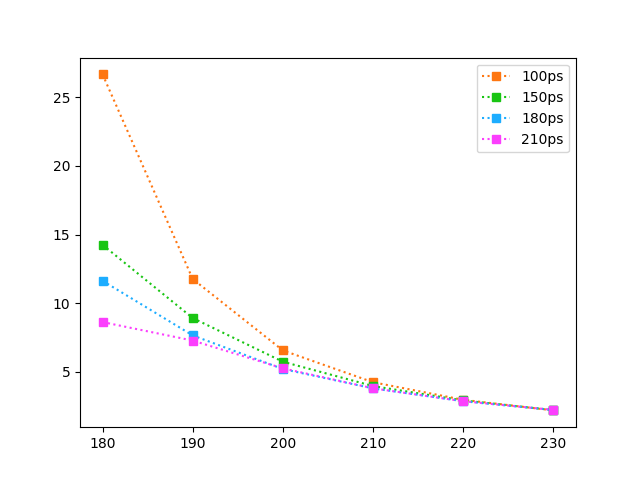
\includegraphics[width=\linewidth]{Batch 3/single Gaussian IRF/2080-err i1.png}
    \captionof{figure}{Std. dev. $I_1$-$I_2=20\%$-$80\%$}
    \label{fig:compirf-Ierr-2080}
\end{minipage}
\begin{minipage}{ .47\linewidth}
    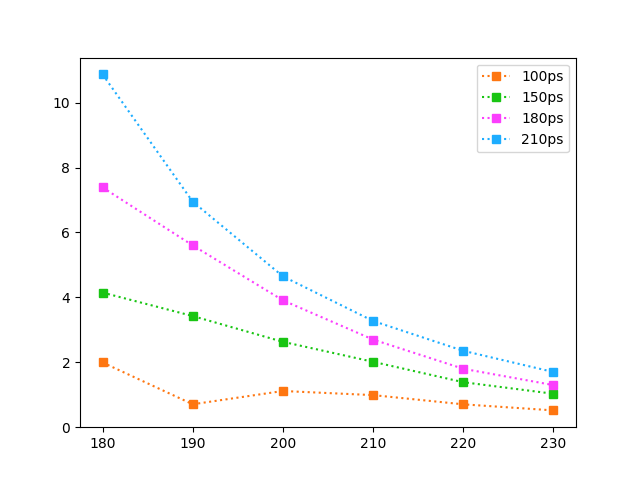
\includegraphics[width=\linewidth]{Batch 3/single Gaussian IRF/5050-diff i1.png}
    \captionof{figure}{$I_1$-$I_2=50\%$-$50\%$}
    \label{fig:compirf-I-5050}
\end{minipage}
\hfill
\begin{minipage}{ .47\linewidth}
    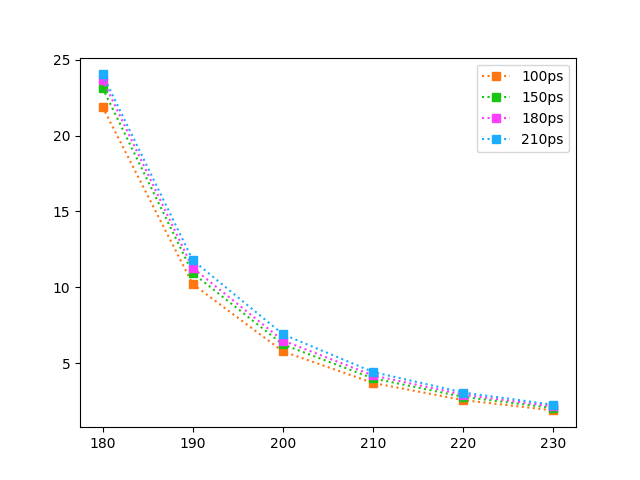
\includegraphics[width=\linewidth]{Batch 3/single Gaussian IRF/5050-err i1.png}
    \captionof{figure}{Std. dev. $I_1$-$I_2=50\%$-$50\%$}
    \label{fig:compirf-Ierr-5050}
\end{minipage}
\begin{minipage}{ .47\linewidth}
    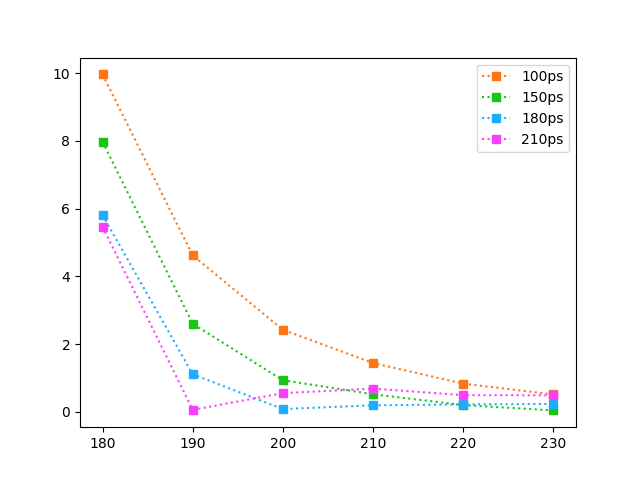
\includegraphics[width=\linewidth]{Batch 3/single Gaussian IRF/8020-diff i1.png}
    \captionof{figure}{$I_1$-$I_2=80\%$-$20\%$}
    \label{fig:compirf-I-8020}
\end{minipage}
\hfill
\begin{minipage}{ .47\linewidth}
    \includegraphics[width=\linewidth]{Batch 3/single Gaussian IRF/8020-err i1.png}
    \captionof{figure}{Std. dev. $I_1$-$I_2=80\%$-$20\%$}
    \label{fig:compirf-Ierr-8020}
\end{minipage}


\section{\boldmath Comparison two component fit, single IRF, 3x Number of counts\unboldmath\label{comp-count}}

\textbf{First component, $\tau_1$}

\begin{minipage}{.47\linewidth}
     
    \includegraphics[width=\linewidth]{Batch 5/t1-diff 2080.png}
    \captionof{figure}{$I_1$-$I_2=20\%$-$80\%$}
    \label{fig:compcount-t1-2080}
\end{minipage}
\hfill
\begin{minipage}{.47\linewidth}
     
    \includegraphics[width=\linewidth]{Batch 5/t1-err 2080.png}
    \captionof{figure}{Std. dev. $I_1$-$I_2=20\%$-$80\%$}
    \label{fig:compcount-t1err-2080}
\end{minipage}
\begin{minipage}{.47\linewidth}
     
    \includegraphics[width=\linewidth]{Batch 5/t1-diff 5050.png}
    \captionof{figure}{$I_1$-$I_2=50\%$-$50\%$}
    \label{fig:compcount-t1-5050}
\end{minipage}
\hfill
\begin{minipage}{.47\linewidth}
     
    \includegraphics[width=\linewidth]{Batch 5/t1-err 5050.png}
    \captionof{figure}{Std. dev. $I_1$-$I_2=50\%$-$50\%$}
    \label{fig:compcount-t1err-5050}
\end{minipage}
\begin{minipage}{.47\linewidth}
     
    \includegraphics[width=\linewidth]{Batch 5/t1-diff 8020.png}
    \captionof{figure}{$I_1$-$I_2=80\%$-$20\%$}
    \label{fig:compcount-t1-8020}
\end{minipage}
\hfill
\begin{minipage}{.47\linewidth}
     
    \includegraphics[width=\linewidth]{Batch 5/t1-err 8020.png}
    \captionof{figure}{Std. dev. $I_1$-$I_2=80\%$-$20\%$}
    \label{fig:compcount-t1err-8020}
\end{minipage}

\vfill
\textbf{Second component, $\tau_2$\unboldmath}

\begin{minipage}{ .47\linewidth}
    \includegraphics[width=\linewidth]{Batch 5/t2-diff 2080.png}
    \captionof{figure}{$I_1$-$I_2=20\%$-$80\%$}
    \label{fig:compcount-t2-2080}
\end{minipage}
\hfill
\begin{minipage}{ .47\linewidth}
    \includegraphics[width=\linewidth]{Batch 5/t2-err 2080.png}
    \captionof{figure}{Std. dev. $I_1$-$I_2=20\%$-$80\%$}
    \label{fig:compcountf-t2err-2080}
\end{minipage}
\begin{minipage}{ .47\linewidth}
    \includegraphics[width=\linewidth]{Batch 5/t2-diff 5050.png}
    \captionof{figure}{$I_1$-$I_2=50\%$-$50\%$}
    \label{fig:compcount-t2-5050}
\end{minipage}
\hfill
\begin{minipage}{ .47\linewidth}
    \includegraphics[width=\linewidth]{Batch 5/t2-err 5050.png}
    \captionof{figure}{Std. dev. $I_1$-$I_2=50\%$-$50\%$}
    \label{fig:compcount-t2err-5050}
\end{minipage}
\begin{minipage}{ .47\linewidth}
    \includegraphics[width=\linewidth]{Batch 5/t2-diff 8020.png}
    \captionof{figure}{$I_1$-$I_2=80\%$-$20\%$}
    \label{fig:compcount-t2-8020}
\end{minipage}
\hfill
\begin{minipage}{ .47\linewidth}
    \includegraphics[width=\linewidth]{Batch 5/t2-err 8020.png}
    \captionof{figure}{Std. dev. $I_1$-$I_2=80\%$-$20\%$}
    \label{fig:compcount-t2err-8020}
\end{minipage}

\pagebreak
\textbf{Intensity}

\begin{minipage}{ .47\linewidth}
    \includegraphics[width=\linewidth]{Batch 5/2080-diff i1.png}
    \captionof{figure}{$I_1$-$I_2=20\%$-$80\%$}
    \label{fig:compcount-I-2080}
\end{minipage}
\hfill
\begin{minipage}{ .47\linewidth}
    \includegraphics[width=\linewidth]{Batch 5/2080-err i1.png}
    \captionof{figure}{Std. dev. $I_1$-$I_2=20\%$-$80\%$}
    \label{fig:compcount-Ierr-2080}
\end{minipage}
\begin{minipage}{ .47\linewidth}
    \includegraphics[width=\linewidth]{Batch 5/5050-diff i1.png}
    \captionof{figure}{$I_1$-$I_2=50\%$-$50\%$}
    \label{fig:compcount-I-5050}
\end{minipage}
\hfill
\begin{minipage}{ .47\linewidth}
    \includegraphics[width=\linewidth]{Batch 5/5050-err i1.png}
    \captionof{figure}{Std. dev. $I_1$-$I_2=50\%$-$50\%$}
    \label{fig:compcount-Ierr-5050}
\end{minipage}
\begin{minipage}{ .47\linewidth}
    \includegraphics[width=\linewidth]{Batch 5/8020-diff i1.png}
    \captionof{figure}{$I_1$-$I_2=80\%$-$20\%$}
    \label{fig:compcount-I-8020}
\end{minipage}
\hfill
\begin{minipage}{ .47\linewidth}
    \includegraphics[width=\linewidth]{Batch 5/8020-err i1.png}
    \captionof{figure}{Std. dev. $I_1$-$I_2=80\%$-$20\%$}
    \label{fig:compcount-Ierr-8020}
\end{minipage}
}

\section{\boldmath Three component fit, $\tau_3=2.6$ns\unboldmath}

\subsection{\boldmath$\tau_1=370, \tau_2=442$\unboldmath}

\begin{minipage}{.47\linewidth}
     
    \includegraphics[width=\linewidth]{Batch 6/3-life/lifetimes.png}
    \captionof{figure}{Three lifetime fit}
    \label{fig:370-440-3life}
\end{minipage}
\hfill
\begin{minipage}{.47\linewidth}
     
    \includegraphics[width=\linewidth]{Batch 6/3-life/intensities.png}
    \captionof{figure}{Intensities, Three lifetimes}
    \label{fig:370-440-3lifeint}
\end{minipage}
\begin{minipage}{.47\linewidth}
     
    \includegraphics[width=\linewidth]{Batch 6/2-life/lifetimes.png}
    \captionof{figure}{Two lifetime fit}
    \label{fig:370-440-2life}
\end{minipage}
\hfill
\begin{minipage}{.47\linewidth}
     
    \includegraphics[width=\linewidth]{Batch 6/2-life/intensities.png}
    \captionof{figure}{Intensities, Two lifetimes}
    \label{fig:370-440-2lifeint}
\end{minipage}
\begin{minipage}{\linewidth}
     
    \includegraphics[width= .47\linewidth]{Batch 6/1-life/lifetime.png}
    \captionof{figure}{One lifetime fit}
    \label{fig:370-440-1life}
\end{minipage}


\vfill
\subsection{\boldmath$\tau_1=355, \tau_2=444$\unboldmath}


\begin{minipage}{.47\linewidth}
     
    \includegraphics[width=\linewidth]{Batch 7/355-444/output/3 life/lifetimes.png}
    \captionof{figure}{Three lifetime fit}
    \label{fig:355-444-3life}
\end{minipage}
\hfill
\begin{minipage}{.47\linewidth}
     
    \includegraphics[width=\linewidth]{Batch 7/355-444/output/3 life/intensities.png}
    \captionof{figure}{Intensities, Three lifetimes}
    \label{fig:355-444-3lifeint}
\end{minipage}
\begin{minipage}{.47\linewidth}
     
    \includegraphics[width=\linewidth]{Batch 7/355-444/output/2 life/lifetimes.png}
    \captionof{figure}{Two lifetime fit}
    \label{fig:355-444-2life}
\end{minipage}
\hfill
\begin{minipage}{.47\linewidth}
     
    \includegraphics[width=\linewidth]{Batch 7/355-444/output/2 life/intensities.png}
    \captionof{figure}{Intensities, Two lifetimes}
    \label{fig:355-444-2lifeint}
\end{minipage}
\begin{minipage}{\linewidth}
     
    \includegraphics[width= .47\linewidth]{Batch 7/355-444/output/1 life/lifetime.png}
    \captionof{figure}{One lifetime fit}
    \label{fig:355-444-1life}
\end{minipage}

\vfill
\subsection{\boldmath$\tau_1=348, \tau_2=440$\unboldmath\label{3lifefits}}


\begin{minipage}{.47\linewidth}
     
    \includegraphics[width=\linewidth]{Batch 7/348-440/output/3 life/lifetimes.png}
    \captionof{figure}{Three lifetime fit}
    \label{fig:348-440-3life}
\end{minipage}
\hfill
\begin{minipage}{.47\linewidth}
     
    \includegraphics[width=\linewidth]{Batch 7/348-440/output/3 life/intensities.png}
    \captionof{figure}{Intensities, Three lifetimes}
    \label{fig:348-440-3lifeint}
\end{minipage}
\begin{minipage}{.47\linewidth}
     
    \includegraphics[width=\linewidth]{Batch 7/348-440/output/2 life/lifetimes.png}
    \captionof{figure}{Two lifetime fit}
    \label{fig:348-440-2life}
\end{minipage}
\hfill
\begin{minipage}{.47\linewidth}
     
    \includegraphics[width=\linewidth]{Batch 7/348-440/output/2 life/intensities.png}
    \captionof{figure}{Intensities, Two lifetimes}
    \label{fig:348-440-2lifeint}
\end{minipage}
\begin{minipage}{\linewidth}
     
    \includegraphics[width= .47\linewidth]{Batch 7/348-440/output/1 life/lifetime.png}
    \captionof{figure}{One lifetime fit}
    \label{fig:348-440-1life}
\end{minipage}
\pagebreak
\chapter{Code}
All code used during this project can be found in the Github repository at this link:
\url{https://github.com/francescotamburi/Palsfit}